\chapter{Creating a new test}
HULTI-GEN provides a step-by-step, test creation setup assistant. This assistant guides you through selecting a test method appropriate for your experiment, setting the parameters for your chosen method, customising the interface\footnote{Currently only available for grading tests}, adding stimuli, and assigning the stimuli into sessions and groups.
\newline\newline
From the main menu, click the 'Create' button to create a new test and begin the setup assistant.

\begin{figure}[ht]
	\centering
	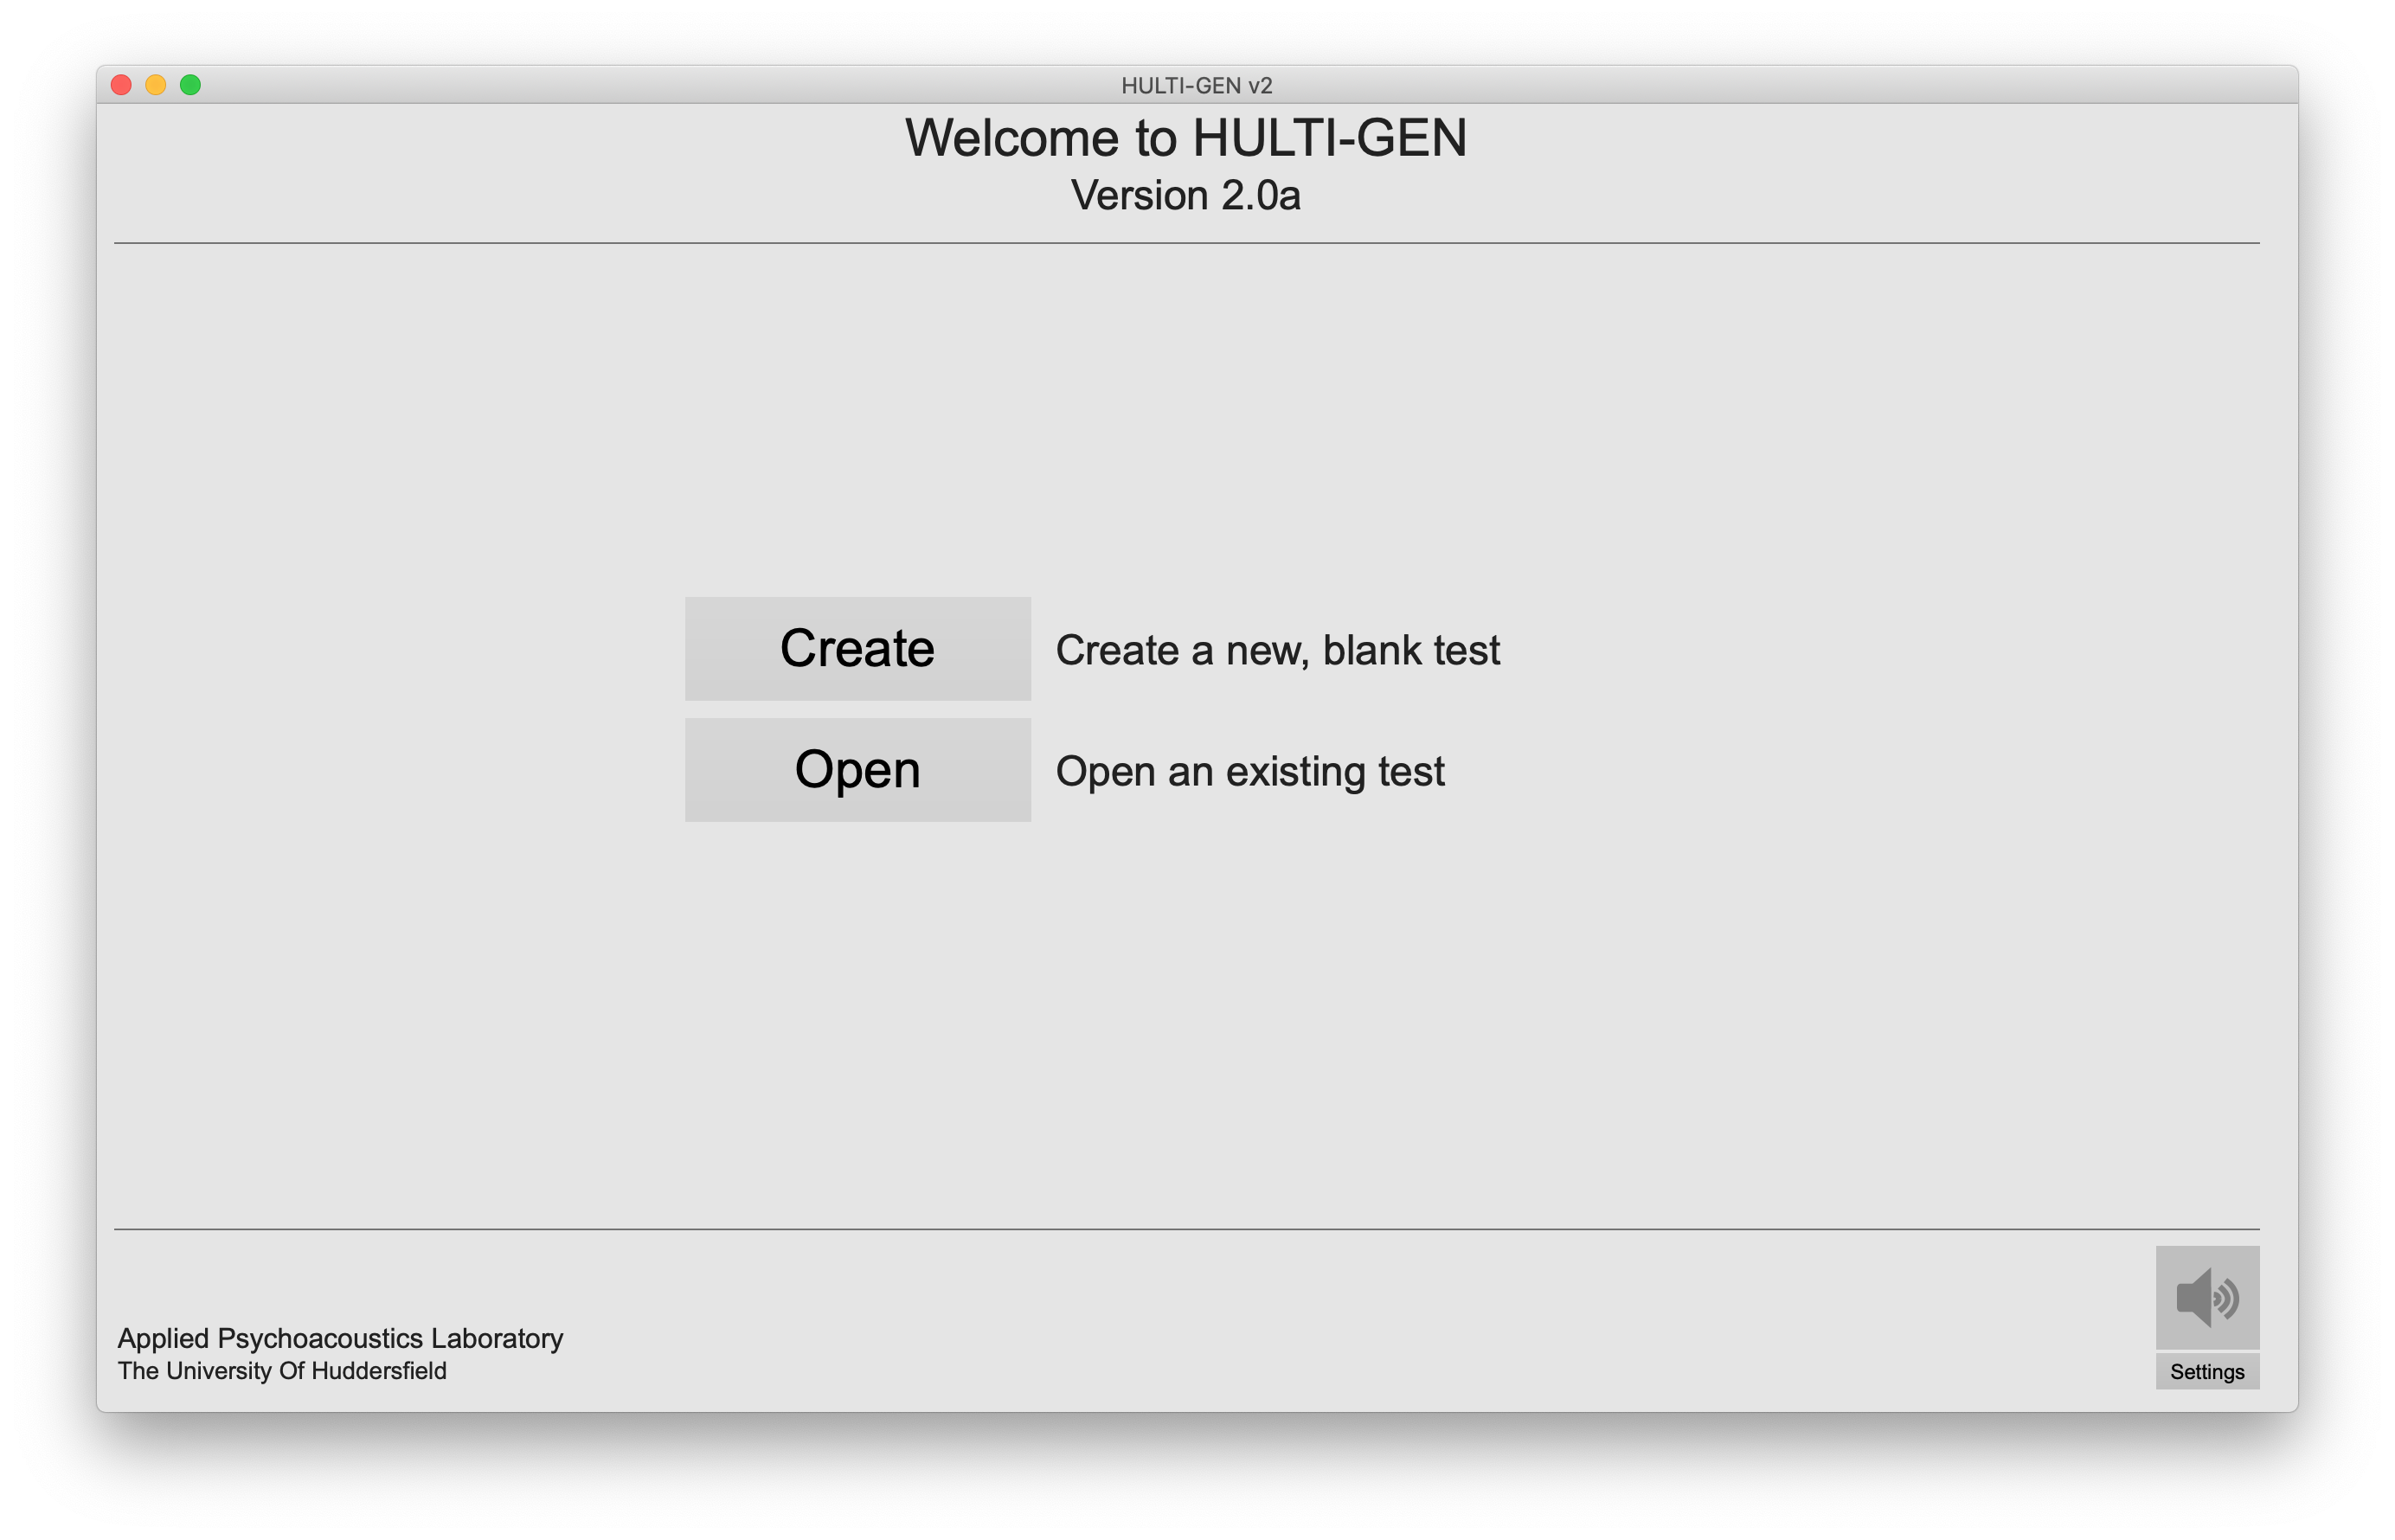
\includegraphics[width=1.0\textwidth]{./images/createTest_step01_mainScreen.png}
	\caption{Click on the 'Create' button to begin the test setup assistant.}
	\label{create::mainScreen}
\end{figure}

On each step of the setup process, you will be greeted by settings or options for that step. Once you have completed a step, click on the 'Next' button to move onto the next step.

\pagebreak

\section{Step 1 - Choose a test method}
When you begin creating a new test, you will be asked what kind of test method, or task, you want subjects to perform, see Figure \ref{create::chooseTest}.

\begin{figure}[ht]
	\centering
	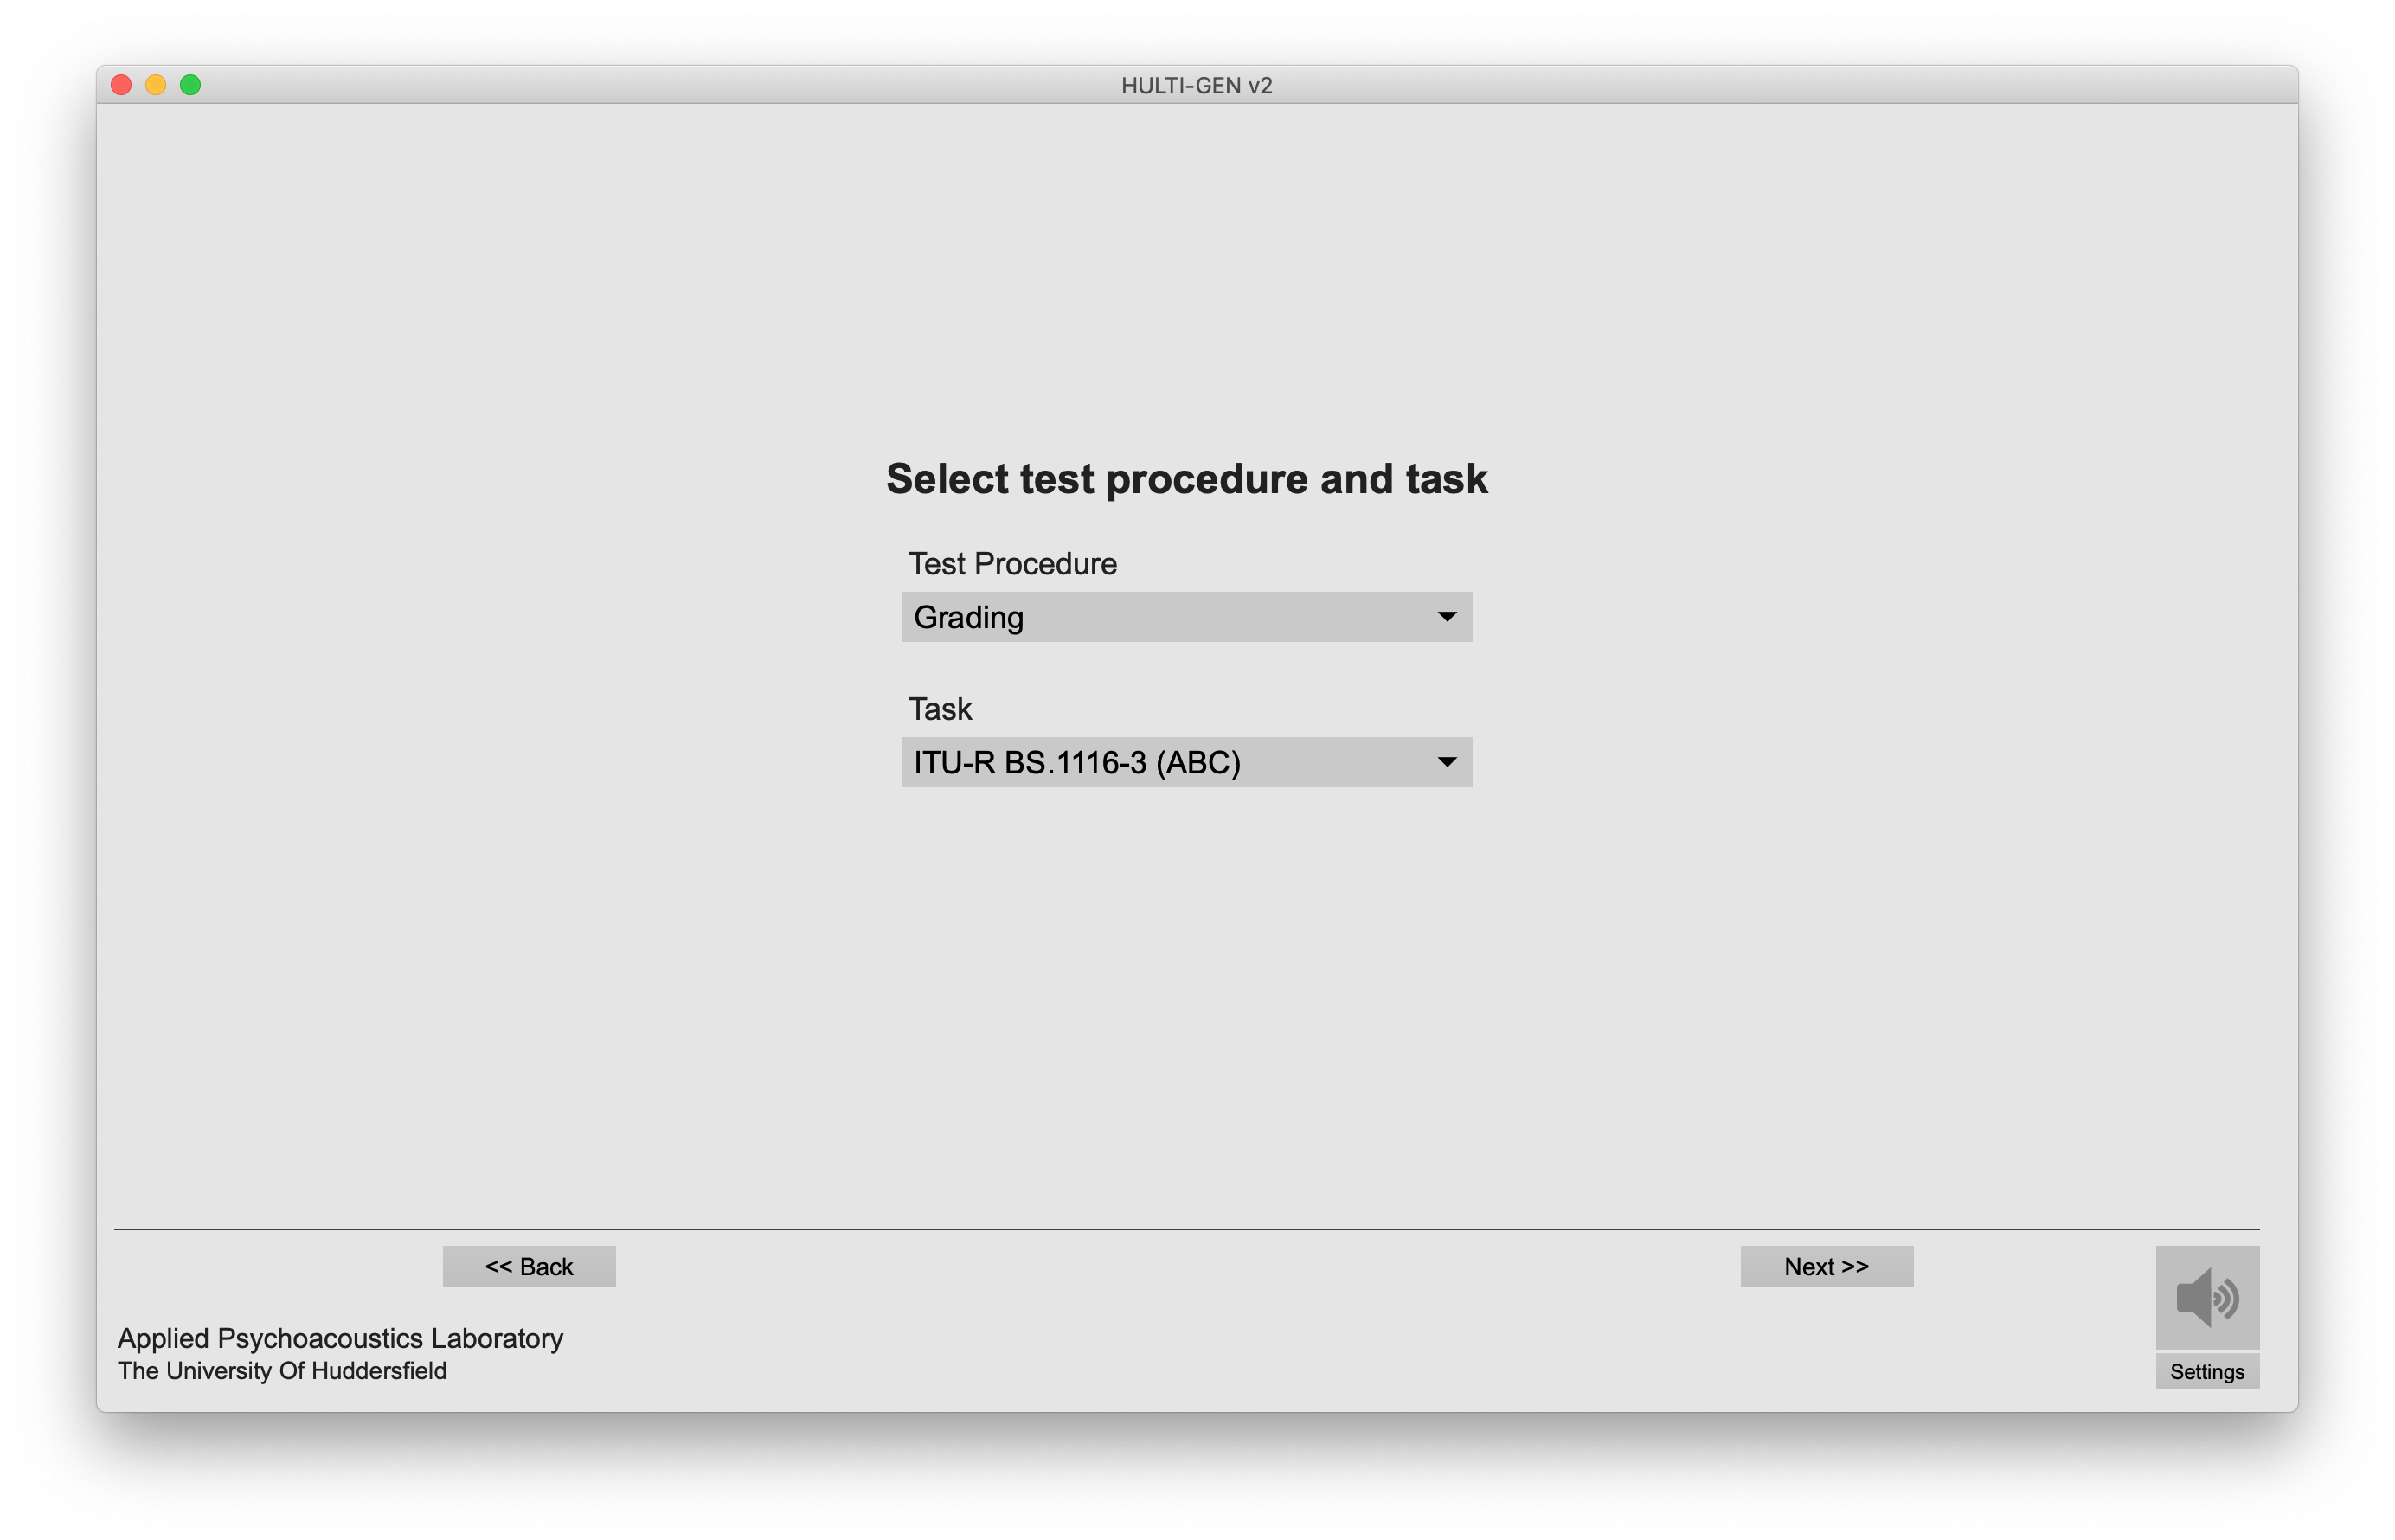
\includegraphics[width=1.0\textwidth]{./images/createTest_step02_chooseTest.png}
	\caption{Choose what type of procedure and task from the on-screen drop-down menus.}
	\label{create::chooseTest}
\end{figure}

Each test method available in HULTI-GEN is grouped by \emph{Procedure} and \emph{Task}. Procedure groups each task by its testing process. Task is specific task the subjects will carry out during the experiment, e.g. MUSHRA. The following table lists all available tasks grouped by their corresponding procedures. Once you have selected a task, click 'Next'.

\begin{center}
	\begin{tabularx}{\textwidth}{|c|X|}
		\hline
		\textbf{Procedure} & \textbf{Task} \\
		\hline
		\multirow{7}*{Grading}
		& ITU-R BS.1116-3 (ABC)\\
		& ITU-R BS.1534-3 (MUSHRA)\\
		& Bipolar $\pm$50 with reference\\
		& ITU-T P.910 Absolute Category Rating (ACR)\\
		& ITU-T P.800 Degradation Category Rating (DCR)\\
		& ITU-T P.800 Comparison Category Rating (CCR)\\
		& 9-Point Hedonic Scale\\
		\hline
		\multirow{4}*{Non-Adaptive Psychophysical}
		& Two-Alternative Forced-Choice (2AFC)\\
		& ABX\\
		& Signal Detection Theory 2AFC\\
		& Signal Detection Theory ABX\\
		\hline
		\multirow{2}*{Adaptive Psychophysical}
		& Staircase 2AFC\\
		& Staircase ABX\\
		\hline
	\end{tabularx}
\end{center}

\section{Step 2 - Input test parameters} 

On this screen you can set the number of sessions, or sittings, and groups of stimuli for the entire test.

\begin{figure}[ht]
	\centering
	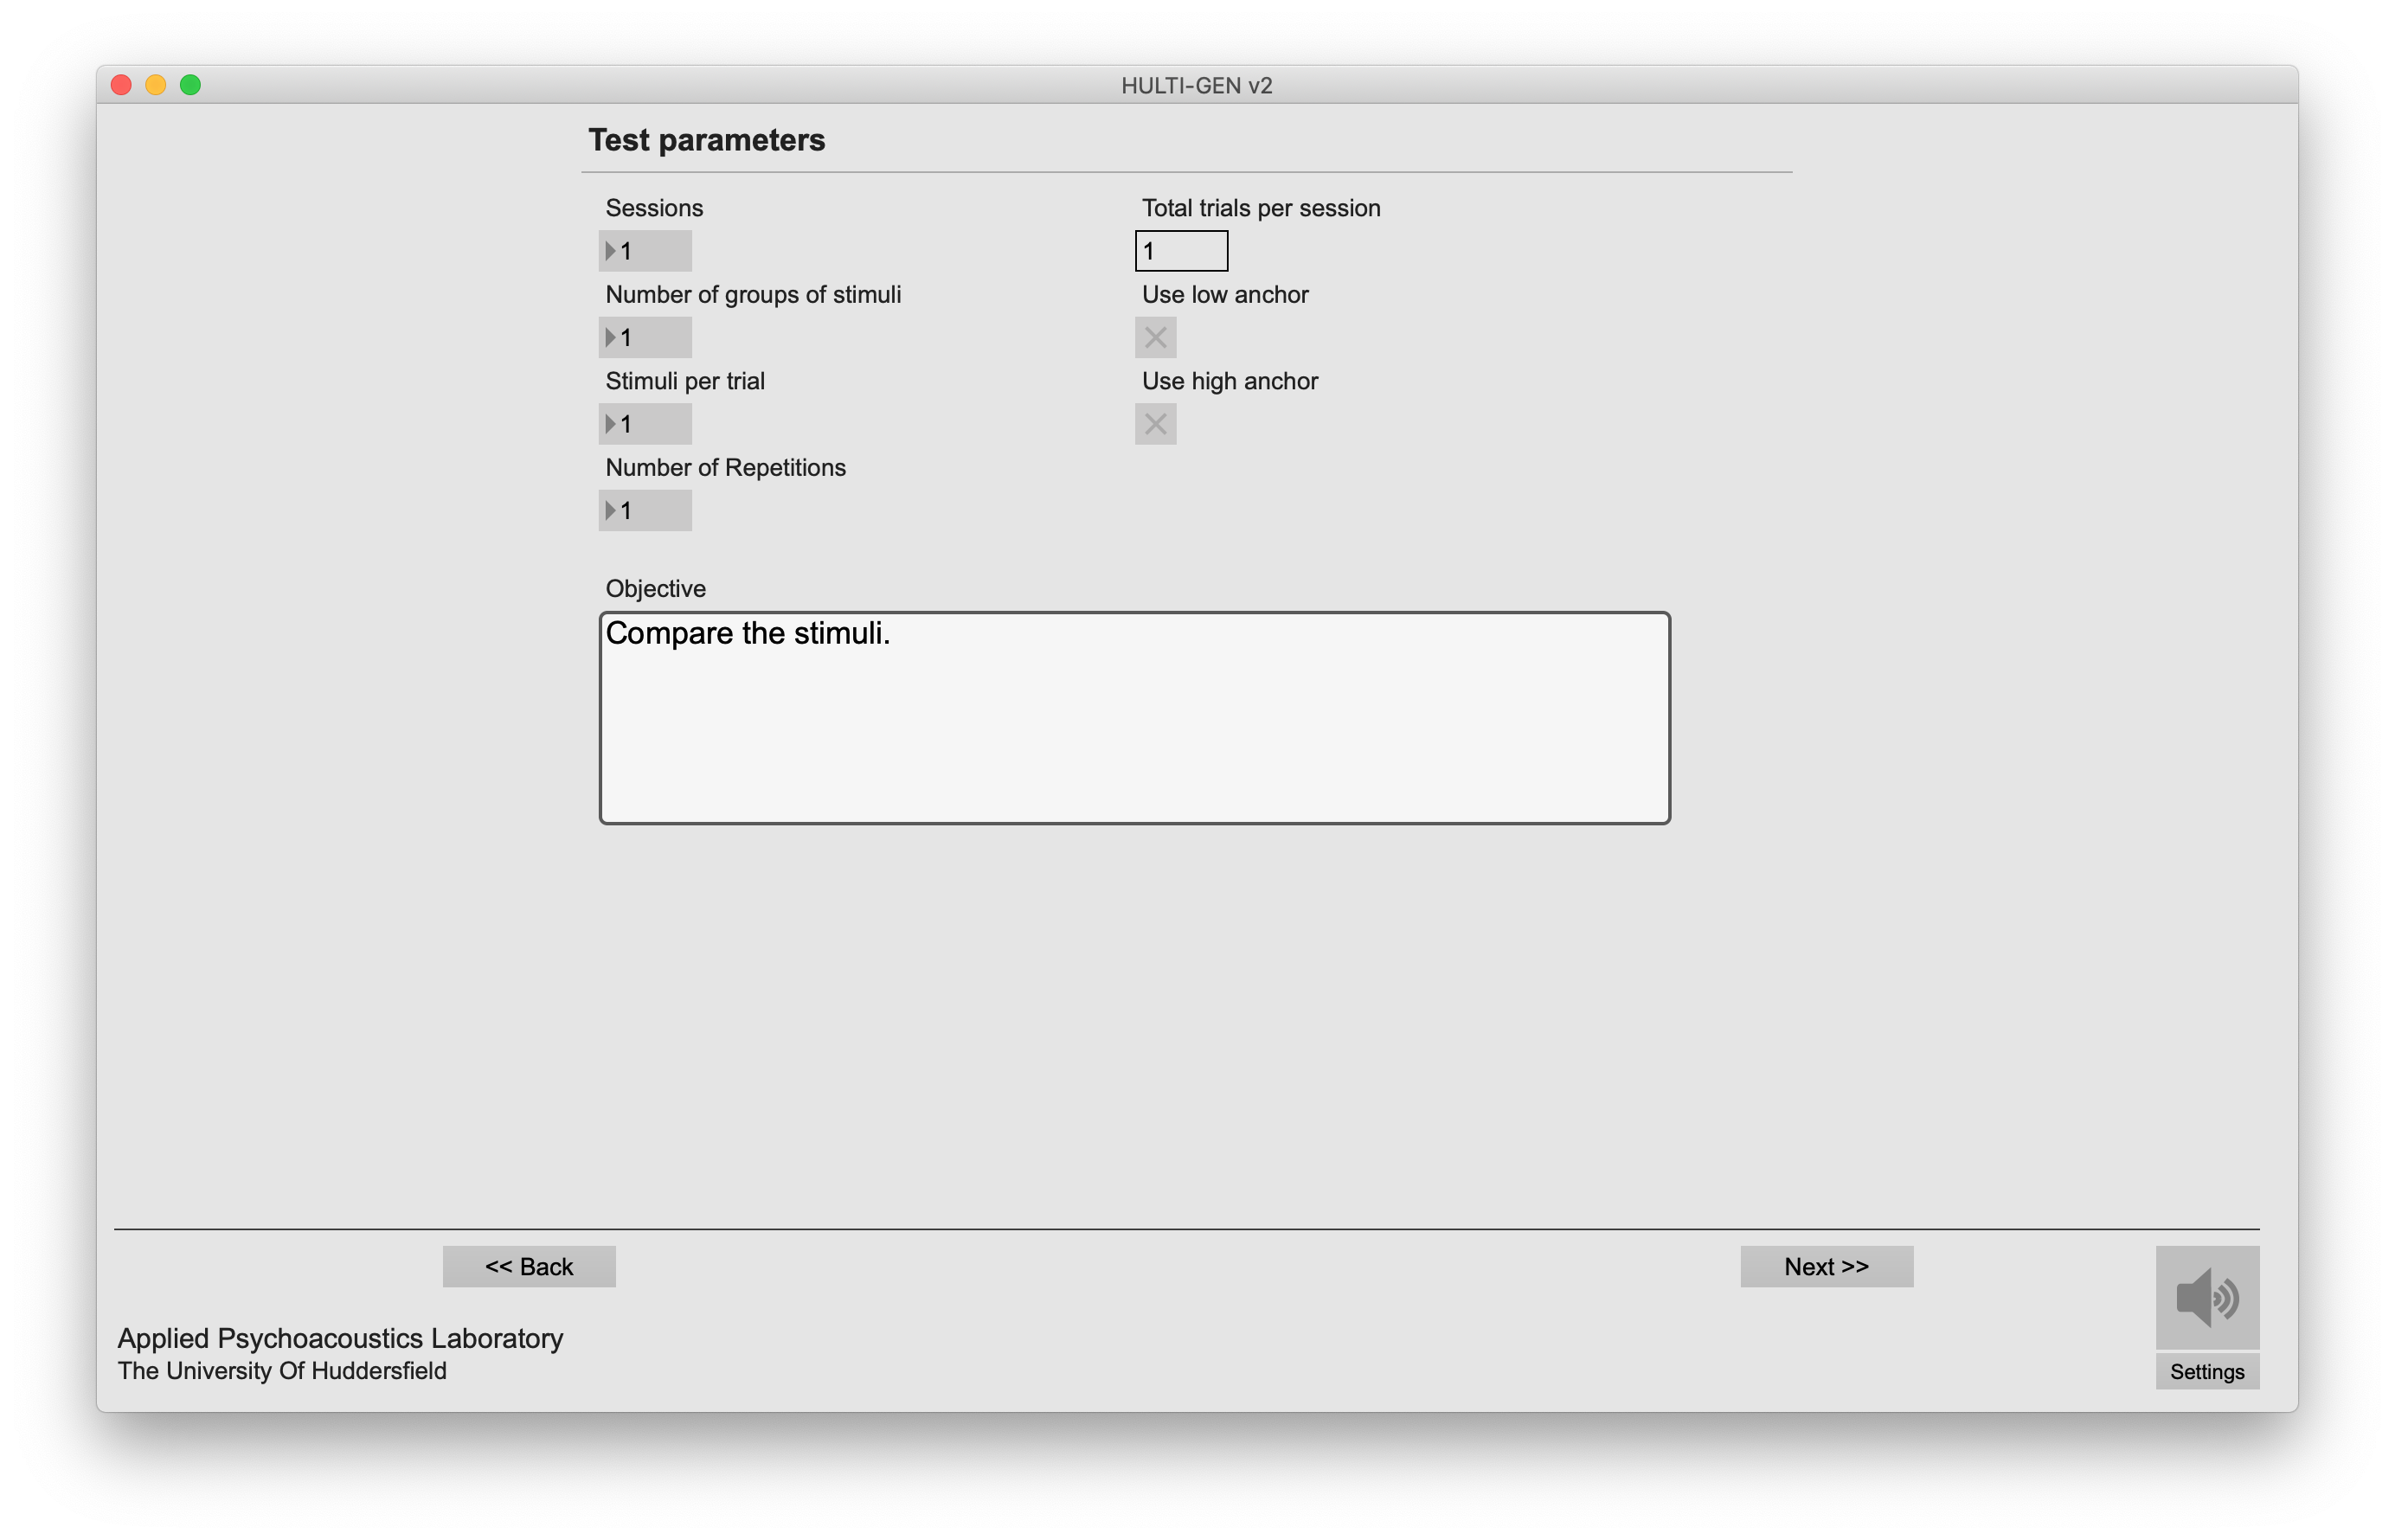
\includegraphics[width=1.0\textwidth]{./images/createTest_step03_testSettings.png}
	\caption{Example test parameters screen.}
	\label{create::testSettings}
\end{figure}

The type settings that you will see are contextual, whereby they depend on the type of procedure that you are configuring. The following list of descriptions explain the settings common to all procedures.

\begin{description}
	\item[Sessions] The number of sittings a subject will undertake for the entire test
	\item[Number of groups of stimuli] Sets the number of stimulus groups per session. In grading tests, this also sets the base number of trials.
	\item[Objective] The instructions that the subject will be shown on screen during the test.
\end{description}

\textit{\textbf{Warning:} If at any point in setup process the number of sessions / groups are changed after being set, assignment of stimuli to any now non-existent sessions / groups will be destroyed.}
\pagebreak

\section{Step 3 - Customise the test interface}

In this step you are able to customise various aspects of the test interface\footnote{\textit{\textbf{Note:} The customisation step is currently only available for grading tasks. Customisation will be made possible for all built-in procedures and tasks in future updates to HULTI-GEN}}. You can edit and resize the labels, change the scale minimum / maximum points and resolution, and (if enabled) position the high and low anchor buttons.

\begin{figure}[ht]
	\centering
	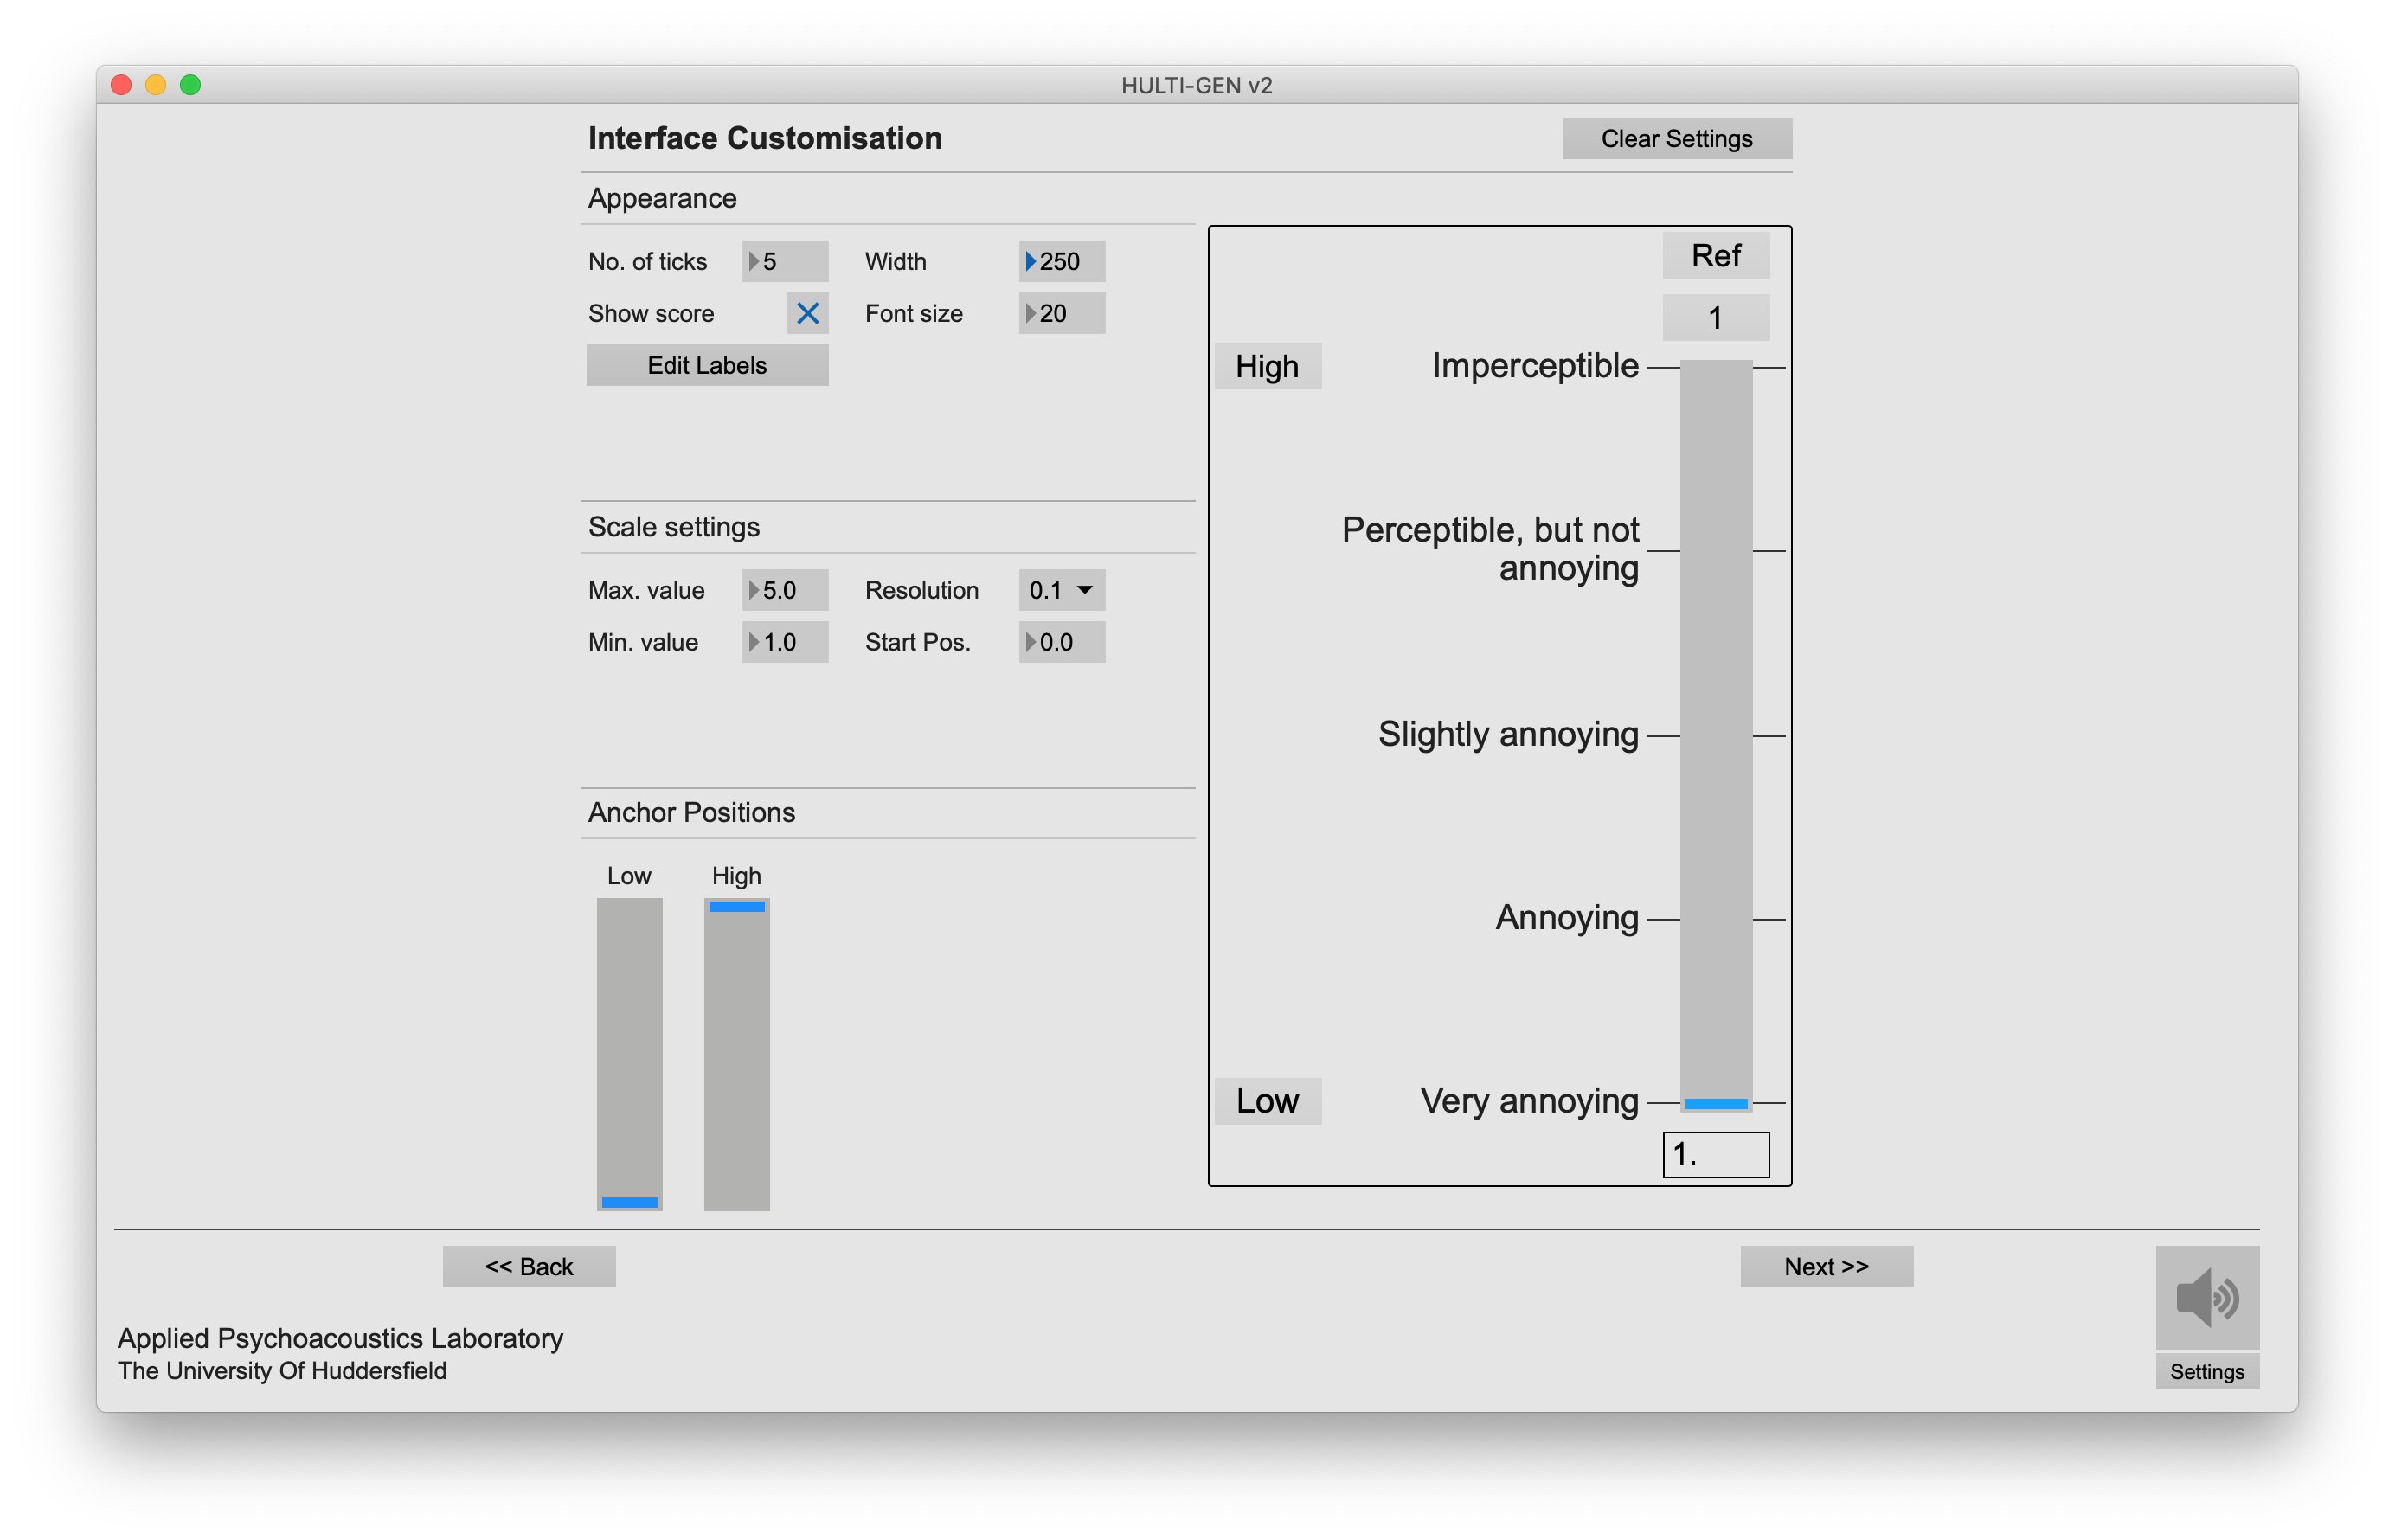
\includegraphics[width=1.0\textwidth]{./images/createTest_step04_customisation.png}
	\caption{Customise the test interface to suit the needs of your experiment.}
	\label{create::customisation}
\end{figure}

\noindent
By default the interface is set to follow the recommendations for the chosen task. Therefore, customising the testing interface means you are working outside of the recommendation. This is not a discouragement, but a reminder that you should justify the design of your test interface where required. After all, the aim of HULTI-GEN is allow experimenters to invent and try new ideas.
\pagebreak

\section{Step 4 - Load stimuli}
Now that the test parameters have been set, it is now time load stimuli. First, the stimuli need to be loaded into a \emph{pool}, which is collection of all the stimuli used throughout the entire test.

\begin{figure}[ht]
	\centering
	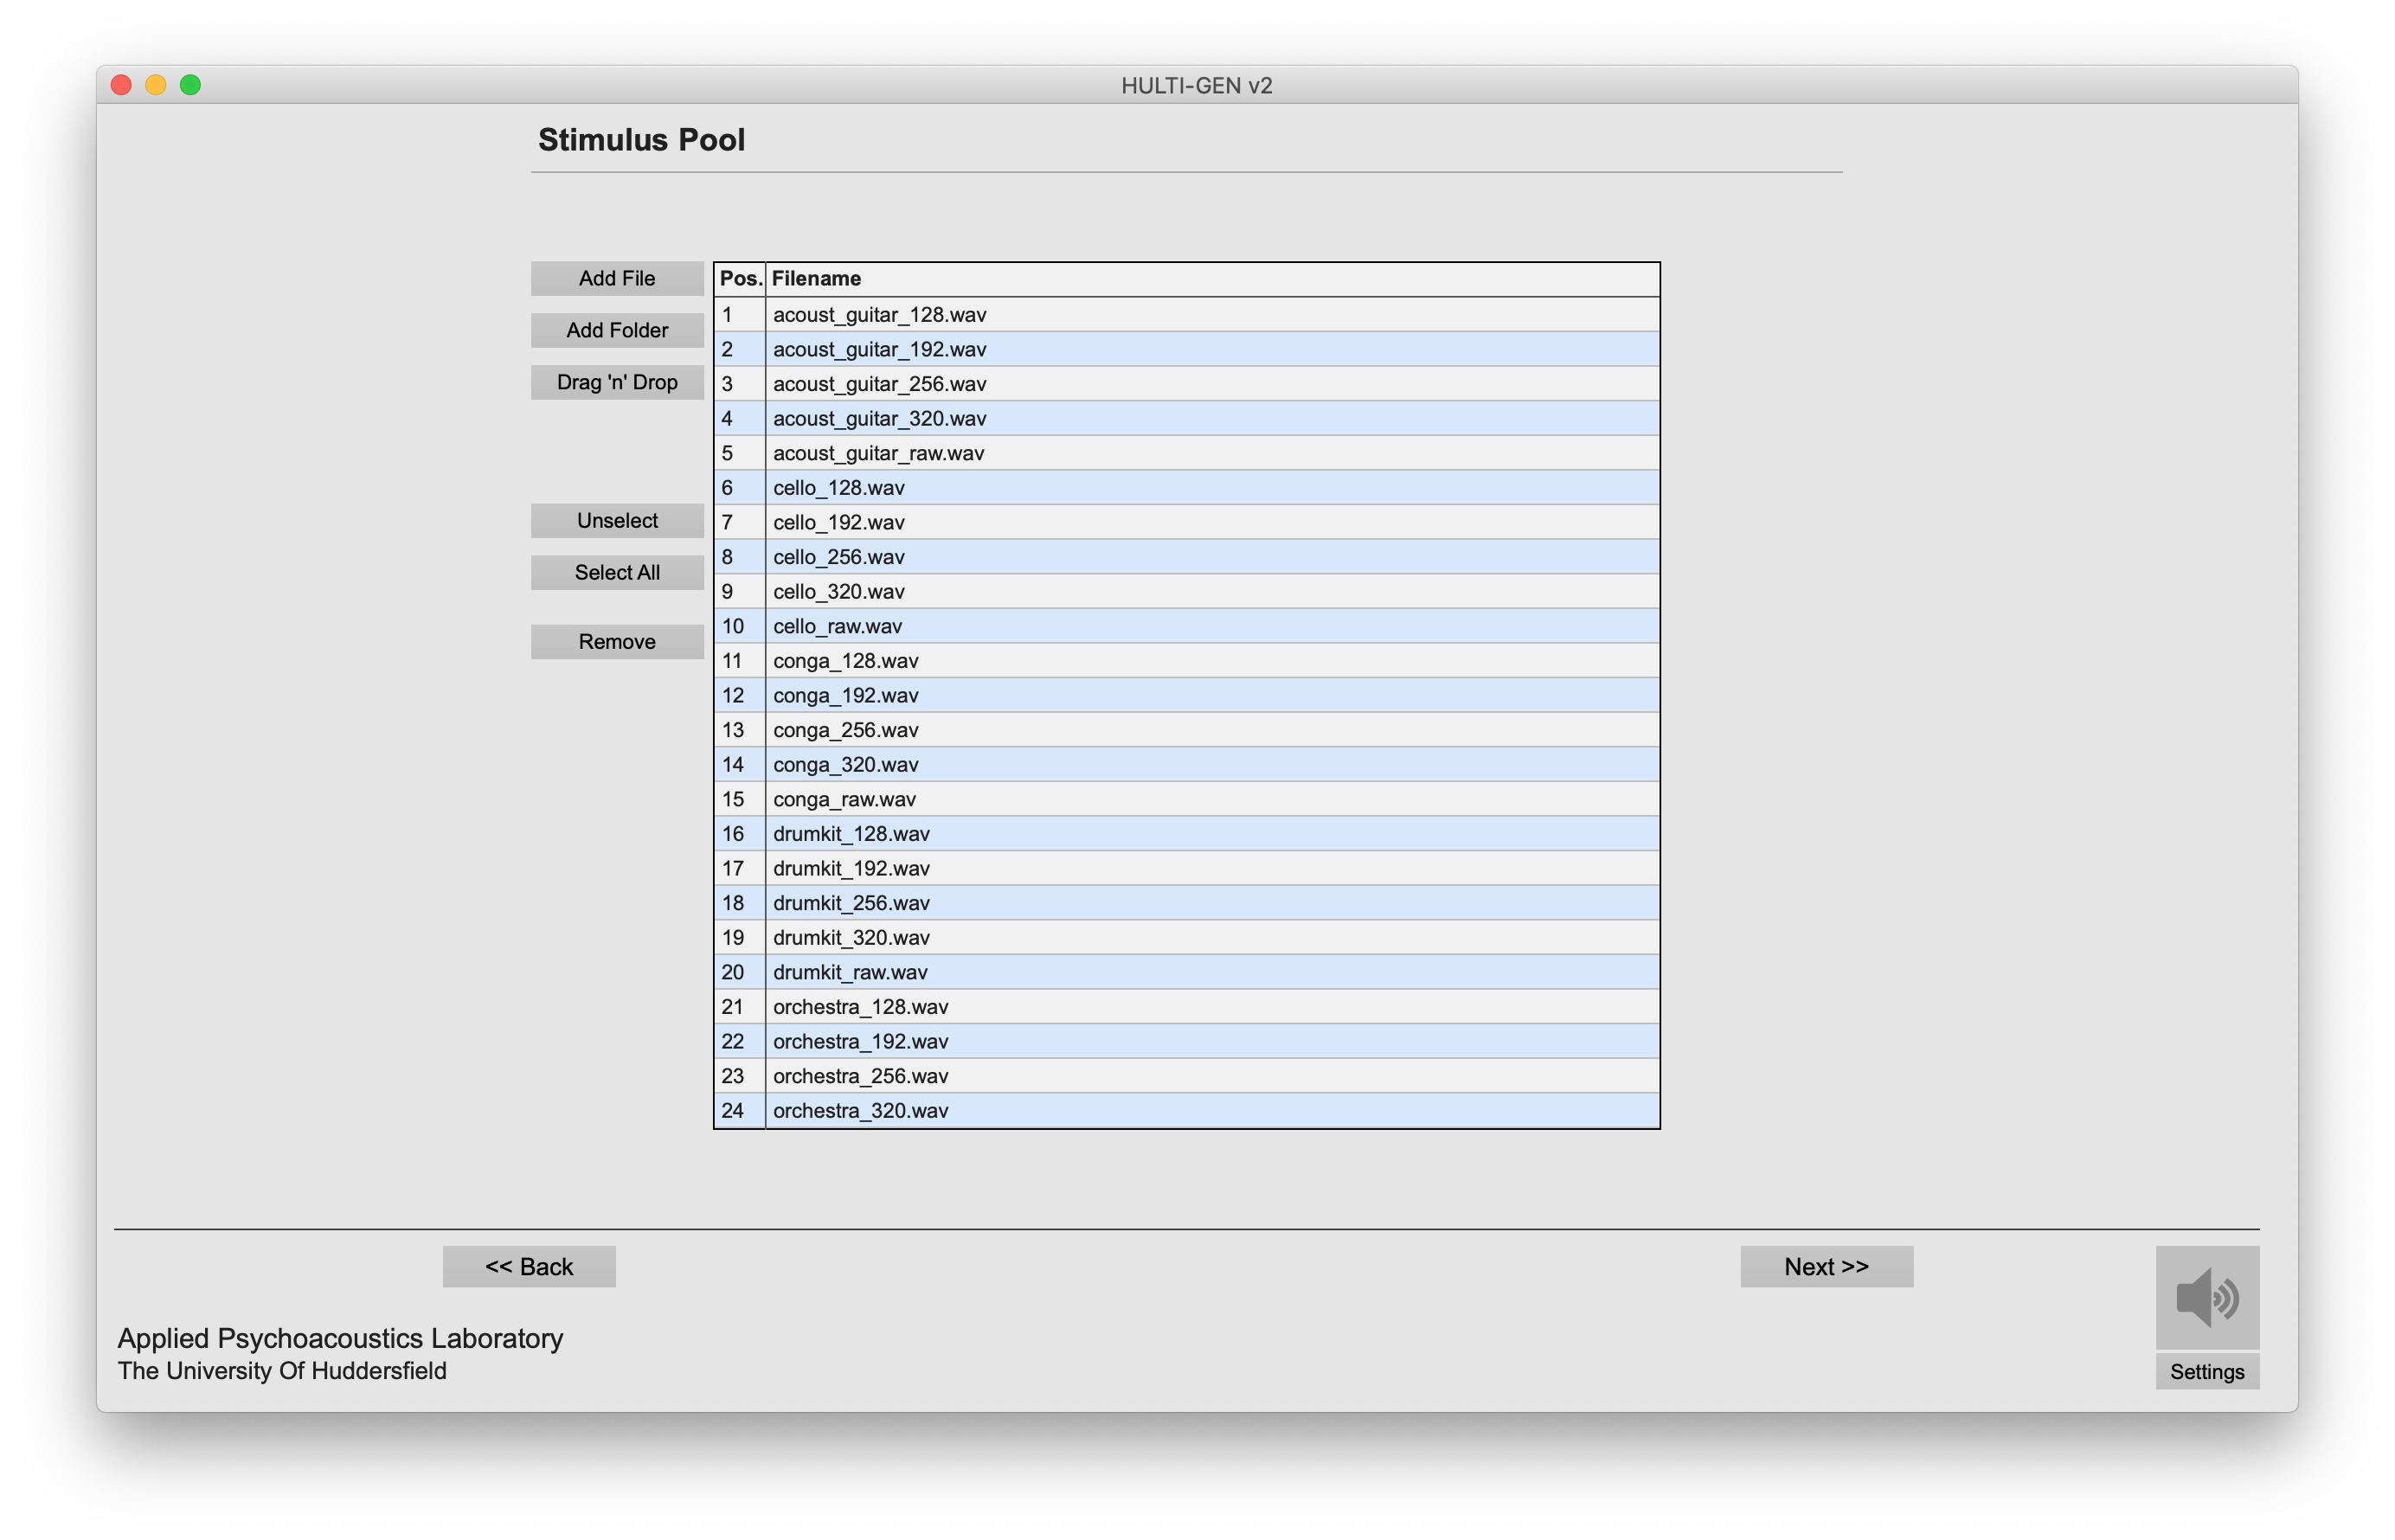
\includegraphics[width=1.0\textwidth]{./images/createTest_step05_stimlusPool.png}
	\caption{Stimuli for the entire test are loaded into a \emph{pool} using this interface.}
	\label{create::stimulusPool}
\end{figure}

\noindent
There are three main ways to add stimuli to the pool.
\begin{description}
	\item[Add File] Browse for and add individual files.
	\item[Add Folder] Add an entire folder of files.
	\item[Drag 'n' Drop] Enable the drag and drop feature of the file-list. When enabled, you can drag files directly onto the file-list, where they are then appended to the list.
\end{description}

\noindent
As you load stimuli into the pool, their filenames are displayed in the file-list in the middle of the screen. Stimuli can be remove by first selecting items in the list, then click 'Remove'. You can select multiple items in the list by holding down 'Cmd' / 'Ctrl' (Operating System dependent) or 'Shift', much like the file browser built into your Operating System.